\documentclass{beamer}

\mode<presentation>
{
	\usetheme{CambridgeUS}
	\setbeamercovered{transparent}
}

\usepackage[spanish]{babel}
\usepackage[latin1]{inputenc}
\usepackage{color}
\usepackage{hyperref}
\usepackage{algorithm,algorithmic}
\usepackage{colortbl}
\usepackage{graphicx}

\title[\textbf{Programaci\'on 2}]{\textbf{Programaci\'on 2}}

\subtitle{Introducci\'on a la Orientaci\'on a Objetos}

\author[Eduardo Godoy]
{
	Profesor: Eduardo Godoy \\
	\vspace{0.5mm}
	\texttt{\normalsize eduardo.gl@gmail.coml} \\ 
	Material elaborado por Rodrigo Olivares \\
	\texttt{\normalsize rodrigo.olivares@uv.cl} \\
}

\institute[Universidad de Valpara\'iso]

%\date{$2^{do}$ Semestre de 2016} 

%\subject{Programaci\'on 2}
%
%\AtBeginSection
%{
%	\begin{frame}<beamer>
%	\frametitle{Contenido}
%	\tableofcontents[currentsection,currentsubsection]
%	\end{frame}
%}
%
%\AtBeginSubsection
%{
%	\begin{frame}<beamer>
%	\frametitle{Contenido}
%	\tableofcontents[currentsection,currentsubsection]
%	\end{frame}
%}
%
%\beamerdefaultoverlayspecification{<+->}

\begin{document}

	\begin{frame}
		\titlepage
	\end{frame}

	\begin{frame}
		\frametitle{Contenido}
		\tableofcontents%[pausesections]
	\end{frame}
	
	\section{Introducci\'on}

		\subsection{Antes de comenzar}

		\begin{frame}
			\frametitle{Introducci\'on}
			\framesubtitle{Antes de comenzar}

			\begin{block}{\textquestiondown Qu\'e es la Orientaci\'on a Objeto?}
  				De manera sintetizada, la orientaci\'on a  objetos es un \textbf{{\em paradigma}} de programaci\'on.
			\end{block}
			\begin{block}{\textquestiondown Qu\'e es un paradigma?}
  				Un paradigma de programaci\'on es un modelo b\'asico de dise\~no y desarrollo de soluciones, con directrices espec\'ificas, tales como: estructura, cohesi\'on, acoploamiento, etc.
			\end{block}
			\begin{exampleblock}{En general}
  				El Paradigma de Orientaci\'on a Objeto es \textbf{una forma} de entender un problema, identificando las principales \textbf{entidades} que se encuentran en \'el.
			\end{exampleblock}
		\end{frame}

		\begin{frame}
			\frametitle{Introducci\'on}
			\framesubtitle{Antes de comenzar}

			\begin{block}{\textquestiondown Qu\'e es un Lenguaje de Programaci\'on?}
  				Es la \textbf{herramienta} seleccionada, para dar soluci\'on al problema detectado.
			\end{block}
			\begin{block}{En relaci\'on a los Lenguaje de Programaci\'on}
  				Se es libre de utilizar la herramienta con la cual se est\'e m\'as habituado. La soluci\'on final no cambia.
			\end{block}
			\begin{exampleblock}{Corolario}
  				El Paradigma de Orientaci\'on a Objeto, no guarda relaci\'on con el Lenguaje de Programaci\'on seleccionado.
			\end{exampleblock}
		\end{frame}

		\begin{frame}
			\frametitle{Introducci\'on}
			\framesubtitle{Antes de comenzar}

			\begin{itemize}
  				\item Tipos de paradigma:
				\begin{itemize}
  					\item \textbf{Procedural o imperativo:}
					\begin{itemize}
  						\item Se decribe como una secuencia instrucciones o comandos que cambian el estado de un programa. El c\'odigo m\'aquina en general est\'a basado en el paradigma imperativo.
					\end{itemize}
					\item \textbf{Declarativo:}
					\begin{itemize}
  						\item Se basa en el \textbf{qu\'e} hacer y no en el c\'omo. Est\'a basado en el desarrollo de programas especificando o \textbf{{\em declarando}} un conjunto de condiciones, proposiciones, afirmaciones, restricciones, ecuaciones o transformaciones que describen el problema y detallan su soluci\'on.
					\end{itemize}
					\item \textbf{L\'ogico:}
					\begin{itemize}
  						\item Se basa en la definici\'on de reglas l\'ogicas para luego, a trav\'es de un motor de inferencias l\'ogicas, responder preguntas planteadas al sistema y as\'i resolver problemas.
					\end{itemize}
				\end{itemize}
			\end{itemize}
		\end{frame}

		\begin{frame}
			\frametitle{Introducci\'on}
			\framesubtitle{Antes de comenzar}

			\begin{itemize}
  				\item Tipos de paradigma:
				\begin{itemize}
					\item \textbf{Estructurado:}
					\begin{itemize}
  						\item La programaci\'on se divide en \textbf{bloques} (procedimientos y funciones) que pueden o no comunicarse entre s\'i. Adem\'as la programaci\'on se controla con secuencia, selecci\'on e iteraci\'on. Su principal ventaja es la \emph{estructura clara} lo que entrega una mejor comprensi\'on de la programaci\'on.
					\end{itemize}
					\item \textbf{Funcional:} 
					\begin{itemize}
  						\item Concibe a la computaci\'on como la evaluaci\'on de funciones aritm\'eticas y evita declarar y cambiar datos. En otras palabras, hace hincapi\'e en la aplicaci\'on de las funciones y composici\'on entre ellas.
					\end{itemize}
					\item \textbf{Orientado a objetos:}
					\begin{itemize}
  						\item Utiliza objetos y sus interacciones, para dise\~nar aplicaciones y programas inform\'aticos. Est\'a basado en varias t\'ecnicas, incluyendo abstracci\'on, encapsulamiento, ocultamiento, herencia, polimorfismo, entre otras.
					\end{itemize}
				\end{itemize}
			\end{itemize}
		\end{frame}

	\subsection{Conceptos}

		\begin{frame}
			\frametitle{Introducci\'on}
			\framesubtitle{Conceptos}

			\begin{exampleblock}{Programaci\'on Orientada a Objeto}
				\begin{itemize}
  					\item[] La \textbf{POO} se basa en la dividir el programa en peque\~nas unidades l\'ogicas de c\'odigo. A estas peque\~nas unidades l\'ogicas de c\'odigo se les denomina \textbf{objetos}. Los objetos son unidades independientes que se comunican entre ellos.\\
					\item[] La \textbf{POO} proporciona t\'ecnicas con las cuales se modela y representa el mundo real (tan fielmente como sea posible).
				\end{itemize}
			\end{exampleblock}
		\end{frame}

		\begin{frame}
			\frametitle{Introducci\'on}
			\framesubtitle{Conceptos}

			\begin{exampleblock}{Qu\'e es un Objeto?}
				\begin{itemize}
  					\item[] Cualquier cosa que vemos a nuestro alrededor. Ej: auto.
					\item[] Un objeto, en general, est\'a compuesto por:
					\begin{itemize}
  						\item Caracter\'isticas / \textbf{atributos} (marca, modelo, color, etc.)
  						\item Comportamiento / \textbf{m\'etodos} (encender, acelerar, frenar, retroceder, etc.)
  					\end{itemize}
				\end{itemize}
			\end{exampleblock}
		\end{frame}
		
		\begin{frame}
			\frametitle{Introducci\'on}
			\framesubtitle{Conceptos}

			\begin{exampleblock}{Objetos y Clases}
				Los programas en POO est\'an construidos en base a objetos con caracter\'isticas (atributos) y comportamiento (m\'etodos) espec\'ificos y que pueden comunicarse entre s\'i.
			\end{exampleblock}
			
			\begin{exampleblock}{}
				\begin{center}
					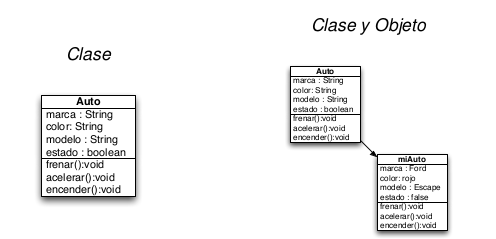
\includegraphics[scale=.5]{images/ClaseAuto.png}
				\end{center}
			\end{exampleblock}
		\end{frame}

		\begin{frame}
			\frametitle{Introducci\'on}
			\framesubtitle{Conceptos}

			\begin{itemize}
  				\item \textbf{Clases:}
				\begin{itemize}
  					\item[] Modelo para m\'ultiples objetos con caracter\'isticas y comportamientos similares. Las clases comprenden todas las caracter\'isticas de una serie particular de objetos. En \textbf{POO} se definen clases como un modelo abstracto de un objeto. En programaci\'on estructurada ser\'ia un tipo de dato (\emph{en C ser\'ia struct o typedef})
				\end{itemize}
				\item \textbf{Instancias:}
				\begin{itemize}
  					\item[] Representaci\'on concreta de un objeto. Al definir una clase se pueden crear muchas instancias de la misma y cada instancia puede tener diferentes caracter\'isticas mientras se comporte y reconozca como objeto de la clase. En programaci\'on estructurada ser\'ia una \emph{variable}.
				\end{itemize}
			\end{itemize}
		\end{frame}

		\begin{frame}
			\frametitle{Introducci\'on}
			\framesubtitle{Conceptos}

			\begin{itemize}
  				\item \textbf{Atributos:}
				\begin{itemize}
  					\item[] Caracter\'isticas que diferencian a un objeto de otro y determinan la ''\emph{forma}'' de ese objeto.
  					\item[] Los atributos se definen como \textbf{variables}. De hecho podr\'ian, ser vistas como \textbf{variables globales del objeto}. Cada instancia de una clase puede tener diferentes valores para sus variables, por lo que a cada variable se le denomina \textbf{variable de instancia}. La clase define el tipo de atributo y cada instancia guarda su propio valor para ese atributo.
				\end{itemize}
			\end{itemize}
		\end{frame}

		\begin{frame}
			\frametitle{Introducci\'on}
			\framesubtitle{Conceptos}

			\begin{itemize}
  				\item \textbf{M\'etodos:}
				\begin{itemize}
  					\item[] Com\'unmente denominadas \textbf{funciones} o \textbf{procedimientos} definidas dentro de una clase, y que operan en sus instancias. Los objetos se \textbf{comunican} entre s\'i mediante el uso \textbf{llamadas a de m\'etodos}. Se dice que una clase puede \textbf{llamar} al m\'etodo de otra clase.
  					\item[] Se pueden definir m\'etodos de instancia (que operan en una instancia de la clase) y los m\'etodos de clase que operan sobre la clase.
				\end{itemize}
			\end{itemize}
		\end{frame}

	\subsection{Principios importantes}

		\begin{frame}
			\frametitle{Introducci\'on}
			\framesubtitle{Principios importantes}

			\begin{itemize}
  				\item \textbf{Abstracci\'on:}
				\begin{itemize}
  					\item Capacidad de analizar y representar las caracter\'isticas esenciales de fen\'omenos complejos.
					\item Una clase es una abstracci\'on o una entidad esencial del problema o la soluci\'on.
					\item Ejemplo: 
					\begin{itemize}
  						\item[] Qu\'e caracter\'isticas tienen de los autos?
  						\item[] Qu\'e comportamiento tienen los autos?
					\end{itemize}
					\item En la \textbf{POO} el concepto de clase es la representaci\'on y el mecanismo por el cual se gestionan las abstracciones. 			
				\end{itemize}
			\end{itemize}
		\end{frame}
		
				
		\begin{frame}
			\frametitle{Introducci\'on}
			\framesubtitle{Principios importantes}

			\begin{itemize}
				\item \textbf{Encapsulamiento:}
				\begin{itemize}
  					\item T\'ecnica para proteger y ocultar el estado interno y el {\em conocimiento} de una entidad.
					\item En el paradigma de la orientaci\'on a objetos, la clase/objeto es la unidad fundamental de encapsulamiento.
					\item En la POO la utilidad del encapsulamiento va por la facilidad de manejar la complejidad, ya que tendremos clases (como cajas negras) donde s\'olo se conoce el comportamiento pero no los detalles internos
				\end{itemize}
			\end{itemize}
		\end{frame}				
				
				
		\begin{frame}
			\frametitle{Introducci\'on}
			\framesubtitle{Principios importantes}

			\begin{itemize}
				\item \textbf{Ocultamiento de informaci\'on:}
				\begin{itemize}
					\item Es la capacidad de ocultar los detalles internos del comportamiento de una clase y exponer s\'olo los detalles que sean necesarios para el resto del sistema.
					\item Cada tipo de objeto expone una \textbf{interfaz} que especifica como pueden interactuar con los objetos de la clase.
  					\item En la \textbf{POO} el objeto pose\'e (al menos) dos vistas:
					\begin{itemize}
  						\item[] Restringir el uso de la clase, pues habr\'a cierto comportamiento \textbf{privado} que no podr\'a ser accedido por otras clases.
						\item[] Controlar el uso de la clase, pues se dar\'an ciertos mecanismos para modificar el estado de una clase.
					\end{itemize}
					\item En Java, el ocultamiento se logra utilizando los modificadores de acceso: public, private y protected delante de las variables y m\'etodo.
				\end{itemize}
			\end{itemize}
		\end{frame}

		\begin{frame}
			\frametitle{Introducci\'on}
			\framesubtitle{Principios importantes}

			\begin{itemize}
				\item \textbf{Herencia:}
				\begin{itemize}
  					\item Organizaci\'on jer\'arquica de clases.
					\item Cada clase tiene una superclase y puede tener una o m\'as subclases. 
					\item Las subclases heredan todos los atributos y m\'etodos de la superclase, esto significa que las subclases incorporan a sus atributos y m\'etodos propios, los atributos y m\'etodos heredados de la superclase.
					\item En Java la herencia se logra usando la palabra reservada: \textbf{extends}. 
					\item En la parte superior de la jerarqu\'ia de clase de Java, est\'a la clase \textbf{Object}. Todas las clases heredan de esta superclase y cada clase hacia abajo agrega m\'as informaci\'on.
				\end{itemize}
			\end{itemize}
		\end{frame}

		\begin{frame}
			\frametitle{Introducci\'on}
			\framesubtitle{Principios importantes}

			\begin{exampleblock}{Jerarqu\'ia de herencia}
				\begin{center}
					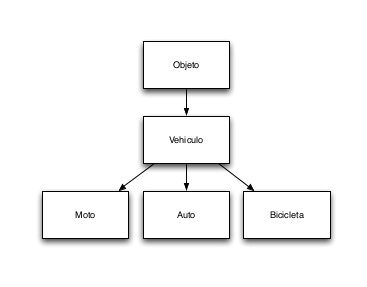
\includegraphics[scale=.5]{images/jerarquia_1.png}
				\end{center}
			\end{exampleblock}
		\end{frame}

		\begin{frame}
			\frametitle{Introducci\'on}
			\framesubtitle{Principios importantes}

			\begin{exampleblock}{Jerarqu\'ia de herencia}
				\begin{center}
					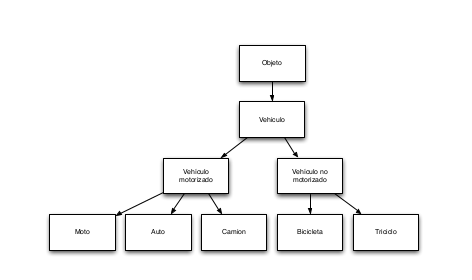
\includegraphics[scale=.55]{images/jerarquia_2.png}
				\end{center}
			\end{exampleblock}
		\end{frame}

		\begin{frame}
			\frametitle{Introducci\'on}
			\framesubtitle{Principios importantes}

			\begin{itemize}
				\item \textbf{Polimorfismo:}
				\begin{itemize}
  					\item Literalmente, \textbf{Poli (muchos/as) - Morphus(formas)}.
  					\item En la \textbf{POO} es la propiedad que le permite a m\'etodos con el mismo nombre implementar distintas funcionalidades, seg\'un las clases donde se apliquen. Es decir, m\'etodos diferentes, asociados a objetos distintos, pueden compartir el mismo nombre. Al llamarlos se utilizar\'a el comportamiento correspondiente al objeto que se est\'e usando.
					\item \textbf{Beneficios:} C\'odigo m\'as gen\'erico. Maximiza la calidad de reuso y extensibilidad.
  					\item \textbf{Ejemplo:}
					\begin{itemize}
						\item Operador \textbf{$+$} para sumar enteros, reales, etc y concatenar cadenas de caracteres.
					\end{itemize}
				\end{itemize}
			\end{itemize}
		\end{frame}

		\begin{frame}
			\frametitle{Introducci\'on}
			\framesubtitle{Principios importantes}

			\begin{itemize}
				\item \textbf{Env\'io de mensajes:}
				\begin{itemize}
  					\item Un objeto es in\'util si est\'a aislado.
  					\item Los objetos de un programa interact\'uan y se comunican entre ellos por medio de \textbf{mensajes}.
  					\item Cuando un \textbf{objeto A} quiere que un \textbf{objeto B} ejecute una de sus funciones (m\'etodos del objeto B), el objeto A \textbf{env\'ia un mensaje} al objeto B. Los mensajes son invocaciones a los m\'etodos de los objetos. 
  					\item Ejemplo: si objeto \emph{miAuto} debe acelerar.
  					\begin{itemize}
  						\item[] El objeto al cual se manda el mensaje (miAuto).
  						\item[] El m\'etodo que debe ejecutar (acelerar()).
  						\item[] Los par\'ametros que necesita ese m\'etodo (10 km/h).
					\end{itemize}
					\item Estas tres partes del mensaje (objeto destinatario, m\'etodo y par\'ametros) son suficiente informaci\'on para que el objeto que recibe el mensaje, ejecute el m\'etodo.
				\end{itemize}
			\end{itemize}
		\end{frame}

	\section{Modelamiento}

		\begin{frame}
			\frametitle{Modelamiento}
			\framesubtitle{Ejemplos}

			\textbf{Modelar las siguientes situaciones}

			\begin{itemize}
				\item[$\rightarrow$] Estacionamiento de autom\'oviles
				\item[$\rightarrow$] Terminal de punto de ventas
				\item[$\rightarrow$] RentaCar (arriendo de veh\'iculos)
				\item[$\rightarrow$] Sistema telef\'onico (Smart-Phone)
				\item[$\rightarrow$] Banca Persona
				\item[$\rightarrow$] Portal de alumnos (UV)
			\end{itemize}
		\end{frame}

	\section{Lenguajes de programaci\'on}

		\subsection{Programar en Java}

		\begin{frame}
			\frametitle{Lenguajes de programaci\'on}
			\framesubtitle{Inicio de Java}

			\begin{exampleblock}{Inicio de Java}
				\begin{itemize}
					\item \textbf{Desarrollado por:} Sun Microsystems en 1991.
					\item \textbf{Propietario actual:} Oracle Corporation desde 2010.
					\item \textbf{Objetivo inicial y actual:}
					\begin{itemize}
						\item Desarrollar un lenguaje de programaci\'on para crear software peque\~nos, r\'apidos, eficientes y port\'atiles para diversos dispositivos de hardware (tel\'efonos celulares, radiolocalizadores y asistentes digitales personales).
						\item Ser el nexo universal que conecte a los usuarios con la informaci\'on que est\'e situada en el computador local, en un servidor Web o en una base de datos.
					\end{itemize}
					\item \textbf{Principio:} \emph{Write Once, Run Everywhere}
				\end{itemize}
			\end{exampleblock}
		\end{frame}

		\begin{frame}
			\frametitle{Lenguajes de programaci\'on}
			\framesubtitle{Caracter\'isticas}

			\begin{exampleblock}{Caracter\'isticas}
				\begin{itemize}
					\item \textbf{Independencia de plataforma}, tanto a nivel del c\'odigo fuente como del binario.
					\item \emph{Diferencia entre c\'odigo fuente y binario?}
					\begin{itemize}
						\item \emph{Independencia en c\'odigo fuente}: los tipos primitivos de datos de Java tienen tama\~no consistentes en todas las plataformas de desarrollo. Las bibliotecas de Java facilitan la escritura del c\'odigo, que puede desplazar se plataforma a plataforma.
						\item \emph{Independencia en binario}: los archivos binarios (bytecodes) pueden ejecutarse en distintas plataformas sin necesidad de volver a compilar la fuente. 
						%\begin{itemize}
						%	\item bytecodes: conjunto de instrucciones ma\'as abstracto que el c\'odigo m\'aquina (c\'odigo intermedio), pero no son especificas a un procesador.
						%\end{itemize}
					\end{itemize}
				\end{itemize}
			\end{exampleblock}
		\end{frame}

		\begin{frame}
			\frametitle{Lenguajes de programaci\'on}
			\framesubtitle{Ventajas}

			\begin{exampleblock}{Ventajas}
				\begin{itemize}
					\item Fomenta la reutilizaci\'on y extensi\'on del c\'odigo.
					\item Permite crear sistemas m\'as complejos.
					\item Relacionar el sistema al mundo real.
					\item Facilita la creaci\'on de programas visuales.
					\item Elimina redundancia a trav\'es de la herencia y polimorfismo
					\item Agiliza el desarrollo de software.
				\end{itemize}
			\end{exampleblock}
		\end{frame}
		
		\begin{frame}
			\frametitle{Lenguajes de programaci\'on}
			\framesubtitle{Ventajas}

			\begin{exampleblock}{Ventajas}
				\begin{itemize}
					\item Facilita el trabajo en equipo.
					\item Facilita el mantenimiento del software.
					\item Recolecci\'on de basura.
					\item En Java no hay punteros (simplicidad).
					\item Las cadenas y los arreglos son objetos reales
					\item La administraci\'on de la memoria es autom\'atica
				\end{itemize}
			\end{exampleblock}
		\end{frame}

		\begin{frame}
			\frametitle{Lenguajes de programaci\'on}
			\framesubtitle{Ambiente de desarrollo Java}

			\begin{exampleblock}{Compilador}
				Genera los ficheros compilados en bytecode (en vez de generar c\'odigo de m\'aquina) (extensi\'on *.class) a partir del co\'digo fuente (extensio\'on *.java). El bytecode ser\'a el conjunto de instrucciones independientes de la plataforma.
			\end{exampleblock}
		\end{frame}
		
		\begin{frame}
			\frametitle{Lenguajes de programaci\'on}
			\framesubtitle{Ambiente de desarrollo Java}

			\begin{exampleblock}{Interprete}
				\emph{Denominado Java Virtual Machine (JVM).} Interpreta el bytecode (c\'odigo neutro) convirtiendo a c\'odigo particular de la CPU utilizada, lo que permite la ejecuci\'on el programa. JVM es una aplicaci\'on que simula una computadora, pero oculta el sistema operativo y el hardware subyacente.
			\end{exampleblock}
		\end{frame}

		\begin{frame}
			\frametitle{Lenguajes de programaci\'on}
			\framesubtitle{Compilaci\'on, interpretaci\'on y ejecuci\'on}

				\begin{center}
					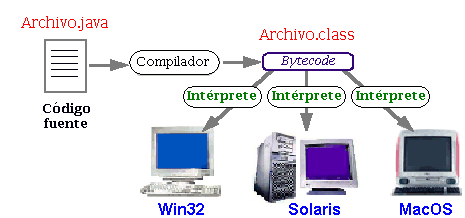
\includegraphics[scale=.65]{images/funcionamiento_java.png}
				\end{center}
		\end{frame}

		\begin{frame}
			\frametitle{Lenguajes de programaci\'on}
			\framesubtitle{Kit de desarrollo Java (JDK)}

			\begin{exampleblock}{Kit de desarrollo Java (JDK)}
				{\scriptsize
				Contiene las herramientas, el conjunto programas y bibliotecas (interfaces de programaci\'on de aplicaciones: APIs) necesarias para desarrollar, compilar y ejecutar programas en Java. 
				\begin{enumerate}
					\item \textbf{javac}: Es el compilador de Java. Se encarga de convertir el c\'odigo fuente escrito en Java a bytecode. Recibe como argumento todos los archivos de c\'odigo fuente (con extension .java). Este comando no es parte de Java Runtine Environment (JRE) dado que JRE esta destinado \'unicamente a ejecutar c\'odigo binario, no permite compilar. Ej: \emph{javac Auto.java}
					\item \textbf{java}: Es el int\'erprete de Java. Ejecuta el bytecode a partir de los archivos con extension .class. Recibe como argumento el nombre del binario ejecutable en formato bytecode sin la extension de archivo .class que identifica de manera visual un binario java. Este comando es parte de JRE y JDK. Ej: \emph{java Auto}
				\end{enumerate}
				}
			\end{exampleblock}
		\end{frame}

		\begin{frame}
			\frametitle{Lenguajes de programaci\'on}
			\framesubtitle{Kit de desarrollo Java (JDK)}

			\begin{exampleblock}{Kit de desarrollo Java (JDK)}
				{\scriptsize
				Contiene las herramientas, el conjunto programas y bibliotecas (interfaces de programaci\'on de aplicaciones: APIs) necesarias para desarrollar, compilar y ejecutar programas en Java. 
				\begin{enumerate}
					\item \textbf{jar}: Herramienta para trabajar con archivos JAR. Permite empaquetar las clases y archivos de Java para fabricar un \'unico archivo contenedor de las aplicaciones, multimedia y
gr\'aficos.  Este comando es parte solo de JDK. Ej: para crear un JAR \emph{jar -cf Auto.jar Auto*}, para extraer un JAR \emph{jar -xf jar\_file}
					\item \textbf{javadoc}: Crea documentaci\'on en formato HTML a partir de el c\'odigo fuente y los comentarios. Ej: \emph{javadoc Auto.java}
					\item \textbf{jdb}: Debugger permite detener la ejecuci\'on del programa en un punto deseado, lo que ayuda la detecci\'on y correcci\'on de errores. Ej: se debe compilar \emph{javac Auto.java} y luego \emph{jdb Auto 10} (debug con punto de interrupci\'on en la l\'inea 10).
				\end{enumerate}
				}
			\end{exampleblock}
		\end{frame}

		\begin{frame}
			\frametitle{Lenguajes de programaci\'on}
			\framesubtitle{Fases para el desarrollo de un programa}

			\begin{exampleblock}{Fases para el desarrollo de un programa}
				{\scriptsize 
				\begin{enumerate}
					\item \textbf{Creaci\'on:} usar un editor para escribir el c\'odigo fuente. Guardarlo con extensi\'on \textbf {.java}. Pueden ser muy \'util utilizar entornos de desarrollo (IDEs).
					\item \textbf{Compilaci\'on:} se usa el comando \textbf {javac}. Ej compilaci\'on: \emph{javac HelloWorld.java}. El resultado de esta fase es un archivo \textbf {.class}
					\item \textbf{Cargar en memoria:} El cargador de memoria toma los archivos \textbf {.class } y los lleva a memoria principal.
					\item \textbf{Verificaci\'on del bytecode:} Verifica que los bytecode sean v\'alidos y no violen restricciones de seguridad.
					\item \textbf{Ejecuci\'on:} La JVM ejecuta los bytecode usando el comando \textbf{java}. Las JVM usan una combinaci\'on de interpretaci\'on y de \emph{compilaci\'on justo a tiempo (JIT).} La JVM analiza el c\'odigo buscando las partes que se ejecutan con frecuencia, para traducirlas al lenguaje de m\'aquina del computador, as\'i cuando encuentra nuevamente el c\'odigo lo ejecuta en lenguaje de m\'aquina que es m\'as r\'apido. As\'i lo programas en java pasan por dos fases de compilaci\'on una para traducir el c\'odigo fuente a bytecode y la otra para traducir el bytecode a lenguaje de m\'aquina. Ej ejecuci\'on: \emph{java HelloWorld}
				\end{enumerate}
				}
			\end{exampleblock}
		\end{frame}

		\subsection{Variables}

		\begin{frame}
			\frametitle{Lenguajes de programaci\'on}
			\framesubtitle{Variables}

			{\scriptsize
			\begin{exampleblock}{Definici\'on}
				\begin{itemize}
  					\item Una \textbf{variable} es un \textbf{nombre} que contiene un valor que puede cambiar a lo largo del programa.
				\end{itemize}
			\end{exampleblock}

			\begin{block}{Tipos principales de variables}
				\begin{itemize}
					\item De acuerdo con el tipo de informaci\'on que contienen, en JAVA hay dos tipos principales de variables:
					\begin{itemize}
						\item {\scriptsize Variables de \textbf{tipos primitivos}. Est\'an definidas mediante un \'unico valor que puede ser \textbf{entero}, de \textbf{punto flotante}, \textbf{car\'acter} o \textbf{booleano}. JAVA permite distinta \textbf{precici\'on} y distintos rangos de valores para estos tipos de variables \textbf{char, byte, short, int, long, float, double, boolean}.}
						\item {\scriptsize Variables \textbf{referencia}. Las variables referencia son referencias o nombres de una informaci\'on m\'as compleja: \textbf{arrays} u \textbf{objetos} de una determinada clase.}
					\end{itemize}
				\end{itemize}
			\end{block}
			}
		\end{frame}

		\begin{frame}
			\frametitle{Lenguajes de programaci\'on}
			\framesubtitle{Variables}

			\begin{block}{Rol de las variables}
				\begin{itemize}
					\item Desde el punto de vista del rol o misi\'on que cumplan en el programa, las variables pueden ser:
					\begin{itemize}
						\item Variables \textbf{miembros} de una clase. Se definen en una clase, fuera de cualquier m\'etodo; pueden ser tipos primitivos o referencias. Com\'unmente son llamados \textbf{atributos} de la clase.
						\item Variables \textbf{locales}. Se definen dentro de un m\'etodo o m\'as en general dentro de cualquier bloque entre llaves \{\}. Se crean en el interior del bloque y se destruyen al finalizar dicho bloque. Pueden ser tambi\'en tipos primitivos o referencias.
					\end{itemize}
				\end{itemize}
			\end{block}
		\end{frame}

		\begin{frame}
			\frametitle{Lenguajes de programaci\'on}
			\framesubtitle{Variables - Nombres de variables}

			\begin{block}{Caracter\'isticas de las variables}
				\begin{itemize}
					\item Los nombres de variables en JAVA se pueden crear con mucha libertad.
					\item Pueden ser cualquier conjunto de caracteres num\'ericos y alfanum\'ericos, sin algunos caracteres especiales utilizados por JAVA como operadores o separadores (\textbf{,.+-*/} etc).
					\item Existe una serie de palabras reservadas las cuales tienen un significado especial para JAVA y por lo tanto no se pueden utilizar como nombres de variables.
				\end{itemize}
			\end{block}
		\end{frame}

		\begin{frame}
			\frametitle{Lenguajes de programaci\'on}
			\framesubtitle{Variables - Palabras reservadas}

			\textbf{Palabras reservadas}
			\begin{center}
				\begin{tabular}{|c|c|c|c|c|c|} \hline
					abstract    & boolean & break         & byte                 & case     & catch        \\ \hline
					char          & class       & const*        & continue         & default & do              \\ \hline
					double     & else         & extends     & final                 & finally   & float \\ \hline
					for             & goto*       & if                 & implements    & import  & instanceof \\ \hline
					int             & interface  & long          & native              & new      & null \\ \hline
					package  & private     & protected & public              & return   & short \\ \hline
					static        & super       & switch       & synchronized & this       & throw \\ \hline
					throws      & transient & try              & void                  & volatile & while \\ \hline
				\end{tabular}
			\end{center}
			\textbf{(*)} son palabras reservadas, pero no se utilizan en la actual implementaci\'on del lenguaje JAVA
		\end{frame}

		\begin{frame}
			\frametitle{Lenguajes de programaci\'on}
			\framesubtitle{Variables -Tipos de datos primitivos}

			\begin{exampleblock}{Caracter\'isticas de las variables}
				Se llaman \textbf{tipos primitivos} de variables de JAVA a aquellas variables sencillas que contienen los tipos de informaci\'on m\'as habituales: valores boolean, caracteres y valores num\'ericos enteros o de punto flotante. 
			\end{exampleblock}
			
			\begin{block}{Caracter\'isticas de las variables}
				\begin{itemize}
					\item Java dispone de \textbf{ocho} tipos primitivos de variables:
					\begin{itemize}
						\item Un tipo para almacenar valores \textbf{true} y  \textbf{false}  \textbf{(boolean)}.
						\item Un tipo para almacenar \textbf{caracteres}  \textbf{(char)}.
						\item Seis tipos para guardar valores \textbf{num\'ericos}.
						\begin{itemize}
							\item Cuatro tipos para \textbf{enteros} \textbf{(byte, short, int y long)}
							\item Dos para valores \textbf{reales de punto flotante} \textbf{(float y double)}.
						\end{itemize}
					\end{itemize}
				\end{itemize}
			\end{block}
		\end{frame}

		\begin{frame}
			\frametitle{Lenguajes de programaci\'on} 
			\framesubtitle{Variables -Tipos de datos primitivos}

			{\scriptsize
			\begin{center}
				\begin{tabular}{|l|l|l|} \hline
					\multicolumn{1}{|>{\columncolor[rgb]{0.8, 0.8, 0.8}}l|}{\textbf{Tipo de variable}} &
					\multicolumn{1}{|>{\columncolor[rgb]{0.8, 0.8, 0.8}}l|}{\textbf{Descripci\'on}} \\ \hline
					\textbf{boolean} & 1 byte. Valores true y false. \\ \hline
					\textbf{char} 	 & 2 bytes. Unicode. Comprende el c\'odigo ASCII. \\ \hline
					\textbf{byte} 	 & 1 byte. Valor entero entre -128 y 127. \\ \hline
					\textbf{Short} 	 & 2 bytes. Valor entero entre -32768 y 32767. \\ \hline
					\textbf{int}		 & 4 bytes. Valor entero entre -2.147.483.648 y
					\\ 			 & 2.147.483.647. \\ \hline
					\textbf{long} 	 & 8 bytes. Valor entre -9.223.372.036.854.775.808 y
					\\			 & 9.223.372.036.854.775.807. \\ \hline
					\textbf{float}	 & 4 bytes (entre 6 y 7 cifras decimales equivalentes). 
					\\ 			 & De -3.402823E38 a -1.401298E-45 y de 1.401298E-45 a 
					\\			 & 3.402823E38. \\ \hline
					\textbf{double}	 & 8 bytes (unas 15 cifras decimales equivalentes). 
					\\ 			 & De -1.79769313486232E308 a -4.94065645841247E-324
					\\ 			 & y de 4.94065645841247E-324 a 1.79769313486232E308. \\ \hline
				\end{tabular}
			\end{center}
			}
		\end{frame}

		\begin{frame}
			\frametitle{Lenguajes de programaci\'on} 
			\framesubtitle{Variables -Tipos de datos primitivos}

			Los tipos primitivos de JAVA tienen algunas caracter\'isticas importantes:

			\begin{itemize}
				\item El tipo \textbf{boolean} no es un valor num\'erico.
				\begin{itemize}
					\item S\'olo admite los valores \textbf{true} o \textbf{false}. 
					\item El tipo boolean no se identifica con el igual o distinto de cero, como en otros lenguajes.
					\item El resultado de la expresi\'on l\'ogica que aparece como condici\'on en un bucle o en una bifurcaci\'on debe ser boolean.
				\end{itemize}
				\item El tipo \textbf{char} contiene caracteres en c\'odigo UNICODE (que incluye el c\'odigo ASCII), y ocupan 16 bits (2 bytes) por car\'acter. Comprende los caracteres de pr\'acticamente todos los idiomas.
			\end{itemize}
		\end{frame}
		
		\begin{frame}
			\frametitle{Lenguajes de programaci\'on} 
			\framesubtitle{Variables -Tipos de datos primitivos}

			Los tipos primitivos de JAVA tienen algunas caracter\'isticas importantes:

			\begin{itemize}
				\item Los tipos \textbf{byte, short, int y long} son n\'umeros enteros que pueden ser positivos o negativos, con distintos valores m\'aximos y m\'inimos. A diferencia de otros lenguajes, en JAVA no hay enteros \textbf{unsigned}.
				\item Los tipos \textbf{float} y \textbf{double} son valores de punto flotante (n\'umeros reales) con 6-7 y 15 cifras decimales exactas (significativos), respectivamente.
				\item Se utiliza la palabra 	\textbf{void} para indicar la ausencia de un tipo de variable determinado.
			\end{itemize}
		\end{frame}
		
		\begin{frame}
			\frametitle{Lenguajes de programaci\'on} 
			\framesubtitle{Variables -Tipos de datos primitivos}

			Los tipos primitivos de JAVA tienen algunas caracter\'isticas importantes:

			\begin{itemize}
				\item A diferencia de otros lenguajes, los tipos de variables en JAVA est\'an perfectamente definidos en todas y cada una de las posibles plataformas. Por ejemplo, un int ocupa siempre la misma memoria y tiene el mismo rango de valores, en cualquier tipo de ordenador.
				\item Existen extensiones de JAVA para aprovechar la arquitectura de los procesadores Intel, que permiten realizar operaciones de punto flotente con una precisi\'on extendida de 80 bits (10 bytes).
			\end{itemize}
		\end{frame}

		\begin{frame}
			\frametitle{Lenguajes de programaci\'on} 
			\framesubtitle{Variables - Definici\'on de variables}

			Definici\'on de variables en JAVA.

			\begin{itemize}
				\item Una variable se define especificando el tipo y el nombre de dicha variable.
				\item Estas variables pueden ser tanto de tipos primitivos como referencias a objetos de alguna clase.
				\item Si no se especifica un valor en su declaraci\'on, las variables primitivas deber\'an ser inicializadas antes de su uso, sino, JAVA no reconocer\'a la variable en el contexto actual.
			\end{itemize}
		\end{frame}

		\begin{frame}
			\frametitle{Lenguajes de programaci\'on} 
			\framesubtitle{Variables - Definici\'on de variables}

			Definici\'on de variables en JAVA.

			\begin{itemize}
				\item Es importante distinguir entre la \textbf{referencia} a un objeto y el \textbf{objeto} mismo.
				\item Una referencia es una variable que indica d\'onde est\'a guardado un objeto en la memoria del ordenador.
				\begin{itemize}
					\item A diferencia de otros lenguajes, JAVA no permite acceder al valor de la direcci\'on, pues en este lenguaje se han eliminado los \textbf{punteros}.
				\end{itemize}
				\item Al declarar una referencia, \'esta a\'un no se encuentra ''apuntando'' a ning\'un objeto en particular y por eso se le asigna el valor \textbf{null}.
				\item Si se desea que esta referencia apunte a un nuevo objeto es necesario crear el objeto utilizando el operador \textbf{new}. Este operador reserva en la memoria del ordenador espacio para ese objeto. 
			\end{itemize}
		\end{frame}

		\begin{frame}
			\frametitle{Lenguajes de programaci\'on} 
			\framesubtitle{Variables - Visibilidad y vida de las variables}

			\begin{block}{Definici\'on}
				\begin{itemize}
					\item Se entiende por \textbf{visibilidad, \'ambito, alcance o scope} de una variable, el fragmento o parte de la aplicaci\'on donde dicha variable es accesible y por lo tanto puede ser utilizada en una expresi\'on.
					\item En JAVA todas las variables deben estar incluidas en una clase.
					\item En general las variables declaradas dentro de unas llaves \{\}, es decir dentro de un bloque, son visibles y existen dentro de estas llaves. 
				\end{itemize}
			\end{block}
		\end{frame}

		\subsection{Operadores}

		\begin{frame}
			\frametitle{Lenguajes de programaci\'on} 
			\framesubtitle{Operadores - Aritm\'eticos}

			\begin{block}{Operadores aritm\'eticos}
				\begin{itemize}
					\item[$\rightarrow$] Son operadores binarios (requieren siempre dos operandos) que realizan las operaciones aritm\'eticas habituales: \textbf{suma} (+), \textbf{resta} (-), \textbf{multiplicaci\'on} (*), \textbf{divisi\'on} (/) y \textbf{resto de la divisi\'on} (\%).
				\end{itemize}
			\end{block}
		\end{frame}

		\begin{frame}
			\frametitle{Lenguajes de programaci\'on} 
			\framesubtitle{Operadores - Asignaci\'on}

			\begin{block}{Operadores de asignaci\'on}
				\begin{itemize}
					\item Los operadores de asignaci\'on permiten asignar un valor a una variable.
					\item El operador de asignaci\'on por excelencia es el operador \textbf{igual} (=). 
					\item La forma general de las sentencias de asignaci\'on con este operador es:
					\begin{itemize}
						\item \textbf{variable} = \textbf{expresion};
					\end{itemize}
					\item JAVA dispone de otros operadores de asignaci\'on. Se trata de las versiones abreviadas del operador (=) que realizan operaciones ''acumulativas'' sobre una variable.
				\end{itemize}
			\end{block}
		\end{frame}

		\begin{frame}
			\frametitle{Lenguajes de programaci\'on} 
			\framesubtitle{Operadores - Asignaci\'on acumulativas}

			\begin{center}
				\begin{tabular}{|l|l|l|} \hline
					\multicolumn{1}{|>{\columncolor[rgb]{0.8, 0.8, 0.8}}c|}{\textbf{Operador}} &
					\multicolumn{1}{|>{\columncolor[rgb]{0.8, 0.8, 0.8}}c|}{\textbf{Uso}} &
					\multicolumn{1}{|>{\columncolor[rgb]{0.8, 0.8, 0.8}}c|}{\textbf{Expesi\'on equivalente}} \\ \hline
					\textbf{$+=$}	& op1 \textbf{$+=$} op2 	& op1 $=$ op1 $+$ op2 \\ \hline
					\textbf{$-=$}	& op1 \textbf{$-=$} op2 	& op1 $=$ op1 $-$ op2  \\ \hline
					\textbf{$*=$} 	& op1 \textbf{$*=$} op2 	& op1 $=$ op1 $*$ op2  \\ \hline
					\textbf{$/=$}	& op1 \textbf{$/=$} op2 	& op1 $=$ op1 $/$ op2  \\ \hline
					\textbf{$\%=$}	& op1 \textbf{$\%=$} op2 	& op1 $=$ op1 $\%$ op2  \\ \hline
				\end{tabular}
			\end{center}
		\end{frame}
		
		\begin{frame}
			\frametitle{Lenguajes de programaci\'on} 
			\framesubtitle{Operadores - Unarios e Instanceof}

			\begin{block}{Operadores unarios}
				Los operadores \textbf{m\'as} (+) y \textbf{menos} (-) unarios sirven para mantener o cambiar el signo de una variable o expresi\'on num\'erica.
			\end{block}

			\begin{block}{Operador \textbf{instanceof}}
				\begin{itemize}
					\item El operador \textbf{instanceof} permite saber si un objeto pertenece o no a una determinada clase.
					\item Es un operador binario cuya forma general es:
					\begin{itemize}
						\item objectName \textbf{instanceof} ClassName
					\end{itemize}
					\item Devuelve \textbf{true o false} seg\'un el objeto pertenezca o no a la clase.
				\end{itemize}
			\end{block}
		\end{frame}

		\begin{frame}
			\frametitle{Lenguajes de programaci\'on} 
			\framesubtitle{Operadores - Condicional \textbf{?}}

			\begin{block}{Operador condicional \textbf{?}}
				\begin{itemize}
					\item Este operador permite realizar bifurcaciones condicionales sencillas.
					\item Su forma general es la siguiente:
					\begin{itemize}
						\item expresionBooleana \textbf{?} respExpresionVerdero : respExpresionFalso
					\end{itemize}
					\item Se eval\'ua \textbf{expresionBooleana} y devuelve \textbf{respExpresionVerdero} si es verdadera o \textbf{respExpresionFalso} si es falsa.
					\item Es el \'unico operador ternario en JAVA (requiere de tres argumentos).
				\end{itemize}
			\end{block}
		\end{frame}

		\begin{frame}
			\frametitle{Lenguajes de programaci\'on} 
			\framesubtitle{Operadores - Incrementales}

			\begin{block}{Operadores incrementales}
				\begin{itemize}
					\item JAVA dispone del operador \textbf{incremento} ($++$) y \textbf{decremento} ($- -$).
					\item El operador ($++$) incrementa en una unidad la variable a la que se aplica, mientras que ($- -$) la reduce en una unidad.
					\item Estos operadores se pueden utilizar de dos formas:
					\begin{itemize}
						\item \textbf{Precediendo}  a la variable \textbf{($++x$)}. En este caso primero se utiliza la variable en la expresi\'on (con el valor actual) y luego se incrementa.
						\item \textbf{Siguiendo} a la variable \textbf{($x++$)}. En este caso primero se incrementa la variable y luego se utiliza (ya incrementada) en la expresi\'on en la que aparece.
					\end{itemize}
				\end{itemize}
			\end{block}
		\end{frame}

		\begin{frame}
			\frametitle{Lenguajes de programaci\'on} 
			\framesubtitle{Operadores - Relacionales}

			\begin{block}{Operadores relacionales}
				\begin{itemize}
					\item Los operadores relacionales sirven para realizar comparaciones de igualdad, desigualdad y relaci\'on de menor o mayor. 
					\item El resultado de estos operadores es siempre un valor \textbf{boolean (true o false)} seg\'un se cumpla o no la relaci\'on considerada. 
					\item Estos operadores se utilizan con mucha frecuencia en las \textbf{bifurcaciones} y en los \textbf{bucles}.
				\end{itemize}
			\end{block}
		\end{frame}

		\begin{frame}
			\frametitle{Lenguajes de programaci\'on} 
			\framesubtitle{Operadores - Relacionales}

			\begin{center}
				\begin{tabular}{|l|l|l|} \hline
					\multicolumn{1}{|>{\columncolor[rgb]{0.8, 0.8, 0.8}}c|}{\textbf{Operador}} &
					\multicolumn{1}{|>{\columncolor[rgb]{0.8, 0.8, 0.8}}c|}{\textbf{Uso}} &
					\multicolumn{1}{|>{\columncolor[rgb]{0.8, 0.8, 0.8}}c|}{\textbf{El resultado es true si:}} \\ \hline
					\textbf{$>$}	& op1 \textbf{$>$} op2 	& op1 es mayor que op2 \\ \hline
					\textbf{$>=$}	& op1 \textbf{$>=$} op2 	& op1 es mayor o igual que op2 \\ \hline
					\textbf{$<$} 	& op1 \textbf{$<$} op2 	& op1 es menor que op2\\ \hline
					\textbf{$<=$}	& op1 \textbf{$<=$} op2 	& op1 es mayor o igual que op2 \\ \hline
					\textbf{$==$}	& op1 \textbf{$==$} op2 	& op1 y op2 son iguales \\ \hline
					\textbf{$!=$}	& op1 \textbf{$!=$} op2 	& op1 y op2 son diferentes \\ \hline
				\end{tabular}
			\end{center}
		\end{frame}

		\begin{frame}
			\frametitle{Lenguajes de programaci\'on} 
			\framesubtitle{Operadores - L\'ogicos}

			\begin{block}{Operadores l\'ogicos}
				\begin{itemize}
					\item Los operadores l\'ogicos se utilizan para construir expresiones l\'ogicas, combinando valores l\'ogicos \textbf{(true y/o false)} o los resultados de los operadores relacionales. 
					\item Debe notarse que en ciertos casos el segundo operando no se eval\'ua porque ya no es necesario (si ambos tienen que ser true y el primero es false, ya se sabe que la condici\'on de que ambos sean true no se va a cumplir). 
					\item Esto puede traer resultados no deseados y por eso se han a\~nadido los operadores (\textbf{\&}) y (\textbf{$\mid$}) que garantizan que los dos operandos se eval\'uan siempre.
				\end{itemize}
			\end{block}
		\end{frame}
		
		\begin{frame}
			\frametitle{Lenguajes de programaci\'on} 
			\framesubtitle{Operadores - L\'ogicos}

			{\scriptsize
			\begin{center}
				\begin{tabular}{|l|l|l|l|} \hline
					\multicolumn{1}{|>{\columncolor[rgb]{0.8, 0.8, 0.8}}c|}{\textbf{Operador}} &
					\multicolumn{1}{|>{\columncolor[rgb]{0.8, 0.8, 0.8}}c|}{\textbf{Nombre}} &
					\multicolumn{1}{|>{\columncolor[rgb]{0.8, 0.8, 0.8}}c|}{\textbf{Uso}} &
					\multicolumn{1}{|>{\columncolor[rgb]{0.8, 0.8, 0.8}}c|}{\textbf{Resultado es true si:}}  \\ \hline
					\textbf{\&\&}		& AND 		& op1 \textbf{\&\&} op2 		& op1 y op2 son true. Si op1 es false 
					\\				&			&						& ya no se eval\'ua op2. \\ \hline
					\textbf{$\mid\mid$}	& OR 		& op1 \textbf{$\mid\mid$} op2 	& op1 y op2 son true. Si op1 es verdadero 
					\\				&			&						& ya no se eval\'ua op2 \\ \hline
					\textbf{$!=$}		& Negaci\'on 	& \textbf{$!$} op 			& op es falso y es falso si op es verdadero 
					\\				&			&						& ya no se eval\'ua op2 \\ \hline
					\textbf{\&}			& AND 		& op1 \textbf{\&} op2 		& op1 y op2 son true. Siempre se eval\'ua op2. \\ \hline
					\textbf{$\mid$}		& OR 		& op1 \textbf{$\mid$}	 op2 		& op1 u op2 son true.  Siempre se eval\'ua op2. \\ \hline
				\end{tabular}
			\end{center}
			}
		\end{frame}

		\begin{frame}
			\frametitle{Lenguajes de programaci\'on} 
			\framesubtitle{Operadores - Concatenaci\'on de caracteres}

			\begin{block}{Operador de concatenaci\'on de car\'ateres}
				\begin{itemize}
					\item El operador \textbf{m\'as (+)} se utiliza tambi\'en para concatenar cadenas de caracteres.
					\item Por ejemplo, para escribir una cantidad con un r\'otulo y unas unidades puede utilizarse la sentencia:
					\begin{itemize}
						\item System.out.println(''El total asciende a '' \textbf{+} totalUnidades );
					\end{itemize}
					\item En el ejemplo anterior, el operador de concatenaci\'on se utiliza para construir la cadena de caracteres que se desea imprimir por medio del m\'otodo \textbf{println()}.
					\item La variable num\'erica \textbf{totalUnidades} es convertida autom\'aticamente por JAVA en cadena de caracteres para poderla concatenar. En otras ocasiones se deber\'a llamar expl\'icitamente a un m\'etodo para que realice esta conversi\'on.
				\end{itemize}
			\end{block}
		\end{frame}

		\subsection{Estructuras de control}

		\begin{frame}
			\frametitle{Lenguajes de programaci\'on}
			\framesubtitle{Estructuras de control}

			{\scriptsize
			\begin{block}{Definici\'on}
				\begin{itemize}
  					\item Facilitan la realizaci\'on de determinadas acciones, mientras que una condici\'on se cumpla. 
					\item Permiten tomar decisiones de \textbf{qu\'e} hacer, en funci\'on de las condiciones que se den en el programa en un momento dado de su ejecuci\'on.
				\end{itemize}
			\end{block}
			\begin{exampleblock}{En JAVA}
				El lenguaje JAVA soporte cuatro tipos de estructuras de control:
				\begin{itemize}
					\item \textbf{Toma de decisi\'on:} if / if-else / switch-case.
					\item \textbf{Bucle o ciclo:} for / while / do-while.
					\item \textbf{Saltos:} break / continue / return / goto.
					\item \textbf{Excepciones.}
				\end{itemize}
			\end{exampleblock}
			}
		\end{frame}

		\begin{frame}
			\frametitle{Lenguajes de programaci\'on}
			\framesubtitle{Estructuras de control - Sentencias condicionales}

			\begin{itemize}
				\item En JAVA la sentencia \textbf{if / if-else}  dota a los programas de la habilidad de ejecutar conjuntos de sentencias seg\'un la condici\'on.
			\end{itemize}

			\begin{block}{La sentencia para \textbf{if} es:}
			{\scriptsize
				\textbf{if} (condici\'on) \textbf{\{} \\
				\hspace{0.3cm} Bloque de sentencias si la condici\'on es \textbf{verdadera}.  \\
				\textbf{\}}
			}
			\end{block}

			\begin{block}{La sentencia para \textbf{if-else} es:}
			{\scriptsize
				\textbf{if} (condici\'on) \textbf{\{} \\
				\hspace{0.3cm} Bloque de sentencias si la condici\'on es \textbf{verdadera}.  \\
				\textbf{\}}\\
				\textbf{else \{}\\
					\hspace{0.3cm} Bloque de sentencias si la condici\'on es \textbf{falsa}.  \\
				\textbf{\}}
			}
			\end{block}
		\end{frame}

		\begin{frame}
			\frametitle{Lenguajes de programaci\'on}
			\framesubtitle{Estructuras de control - Sentencias condicionales}

			\begin{itemize}
				\item Supongamos que un programa debe realizar diferentes acciones dependiendo de si el usuario oprime el bot\'on \textbf{aceptar} o el bot\'on \textbf{cancelar} en una ventana de di\'alogo. Nuestro programa puede realizar esta bifurcaci\'on usando la sentencia \textbf{if-else}:
			\end{itemize}
			
			\begin{block}{Bifurcaci\'on con la sentencia \textbf{if-else}.}
			{\scriptsize
				\textbf{if} (respuesta.equals(''Aceptar'')) \textbf{\{} \\
				\hspace{0.3cm} System.out.println(''Su petici\'on esta siendo atendida'');  \\
				\textbf{\}}\\
				\textbf{else \{}\\
					\hspace{0.3cm} System.out.println(''Cancelando acci\'on'' );  \\
				\textbf{\}}
			}
			\end{block}
		\end{frame}

		\begin{frame}
			\frametitle{Lenguajes de programaci\'on}
			\framesubtitle{Estructuras de control - Sentencias condicionales}

			\begin{itemize}
				\item Se pueden anidar expresiones \textbf{if-else}, para poder implementar aquellos casos con m\'ultiples acciones. Esto es lo que se suele denominar como sentencias \textbf{else-if}.
			\end{itemize}

			\begin{block}{Ejemplo de Bifurcaciones m\'ultiples:}
				\begin{itemize}
					\item Supongamos que se desea escribir un programa que clasifique seg\'un el contenido de una variable denominada \textbf{valor}, asigne una letra a otra variable denominada \textbf{clasificacion}.
					\item A, para un valor entre 100 y 91 (inclusive).
					\item B, para un valor entre 90 y 81 (inclusive).
					\item C, para un valor entre 80 y 71 (inclusive).
					\item F, si no es ninguno de los anteriores.
				\end{itemize}
			\end{block}
		\end{frame}

		\begin{frame}
			\frametitle{Lenguajes de programaci\'on}
			\framesubtitle{Estructuras de control - Sentencias condicionales}

			\begin{block}{Ejemplo de Bifurcaciones m\'ultiples - Soluci\'on}
			{\scriptsize
			\textbf{int} valor;\\
			\textbf{char} clasificacion;\\
			\vspace{0.3cm}
			\textbf{if} (valor $>$ 90 \hspace{0.1cm} \textbf{\&\&} \hspace{0.1cm} valor $<=$ 100) \textbf{\{} \\
  			\hspace{0.3cm} clasificacion = 'A';\\
			\textbf{\}} \\
			\textbf{else if} (valor $>$ 80 \hspace{0.1cm} \textbf{\&\&} \hspace{0.1cm} valor $<$= 90) \textbf{\{} \\
			\hspace{0.3cm} clasificacion = 'B';\\
			\textbf{\}} \\
			\textbf{else if} (valor $>$ 70 \hspace{0.1cm} \textbf{\&\&} \hspace{0.1cm} valor $<$= 80) \textbf{\{} \\
			\hspace{0.3cm} clasificacion = 'C';\\
			\textbf{\}} \\
			\textbf{else} \textbf{\{} \\
			\hspace{0.3cm} clasificacion = 'F';\\
			\textbf{\}}
			}
			\end{block}
		\end{frame}

		\begin{frame}
			\frametitle{Lenguajes de programaci\'on}
			\framesubtitle{Estructuras de control - Sentencias condicionales}

			\begin{itemize}
				\item Este sistema de programaci\'on (else-if) no es recomendable, por la p\'erdida de claridad en la lectura del programa. Por ello el lenguaje JAVA incluye la sentencia \textbf{switch-case}, para dirigir el flujo de control de variables con m\'ultiples valores.
				\item La sentencia \textbf{switch} permite seleccionar entre varias opciones, seg\'un el valor de cierta expresi\'on.
				\item Cada sentencia case debe ser \'unica y el valor que eval\'ua debe ser del mismo tipo que el devuelto por la expresi\'on de la sentencia \textbf{switch}.
				\item Las sentencias \textbf{break} permiten salir del \textbf{switch} y continar con la siguiente instrucci\'on. Las sentencias \textbf{break} son necesarias porque sin ellas se ejecutar\'ian secuencialmente las sentencias \textbf{case} restantes. 
			\end{itemize}
		\end{frame}

		\begin{frame}
			\frametitle{Lenguajes de programaci\'on}
			\framesubtitle{Estructuras de control - Sentencias condicionales}

			\begin{itemize}
				\item Finalmente, se puede usar la sentencia \textbf{default} para manejar los valores que no son expl\'icitamente contemplados por alguna de las sentencias \textbf{case}. Su uso es altamente recomendado.
			\end{itemize}

			\begin{block}{La forma general de la sentencia \textbf{switch} es la siguiente:}
			{\scriptsize
				\textbf{switch} (expresionMultivalor) \textbf{\{} \\
				\hspace{0.3cm} \textbf{case} valor1: \\
				\hspace{0.6cm} bloqueDeSentenciasParaValor1; \\
				\hspace{0.6cm} \textbf{break}; \\
				\hspace{0.3cm} \textbf{case} valor2: \\
				\hspace{0.6cm} bloqueDeSentenciasParaValor2; \\
				\hspace{0.6cm} \textbf{break}; \\
				\hspace{0.3cm}...\\
				\hspace{0.3cm} \textbf{default}: \\
				\hspace{0.6cm} bloqueDeSentenciasParaValorNoDeterminado; \\
				\hspace{0.6cm} \textbf{break}; \\
				\textbf{\}}
			}
			\end{block}
		\end{frame}

		\begin{frame}
			\frametitle{Lenguajes de programaci\'on}
			\framesubtitle{Estructuras de control - Sentencias condicionales}

			\begin{block}{Ejemplo de sentencia \textbf{switch}}
				\begin{itemize}
					\item Supongamos un programa con una variable entera \textbf{meses} cuyo valor indica el mes actual y se desea imprimir el nombre del mes en que estemos. Se puede utilizar la sentencia \textbf{switch} para realizar esta operaci\'on.
					\item Si el valor a comparar no existe o no es un valor v\'alido, el programa debe indicar el error.
					\item Luego de implementar la soluci\'on con la sentencia \textbf{switch}, implementarla con la sentencia \textbf{else-if} y comparar ambas soluciones. 
				\end{itemize}
			\end{block}
		\end{frame}

		\begin{frame}
			\frametitle{Lenguajes de programaci\'on}
			\framesubtitle{Estructuras de control - Sentencias condicionales}

			\begin{block}{Ejemplo de sentencia \textbf{switch} - Soluci\'on}
			{\scriptsize
				\textbf{int} mes;\\
				\vspace{0.3cm}
				\textbf{switch} (mes) \textbf{\{} \\
				\hspace{0.3cm} \textbf{case} 1: \\
				\hspace{0.6cm} System.out.println(''Enero''); \\
				\hspace{0.6cm} \textbf{break}; \\
				\hspace{0.3cm} \textbf{case} 2: \\
				\hspace{0.6cm} System.out.println(''Febrero''); \\
				\hspace{0.6cm} \textbf{break}; \\
				\hspace{0.3cm} //... Otros meses \\
				\hspace{0.3cm} \textbf{default}: \\
				\hspace{0.6cm} System.out.println(''Mes no v\'alido''); \\
				\hspace{0.6cm} \textbf{break}; \\
				\textbf{\}}
			}
			\end{block}
		\end{frame}

		\begin{frame}
			\frametitle{Lenguajes de programaci\'on}
			\framesubtitle{Estructuras de control - Sentencias de iteraci\'on o bucles}

			\begin{itemize}
				\item En Java se reconocen tres tipos de sentencias de iteraci\'on:
				\begin{itemize}
					\item \textbf{while}.
					\item \textbf{do-while}.
					\item	\textbf{for}.
				\end{itemize}
			\end{itemize}
		\end{frame}

		\begin{frame}
			\frametitle{Lenguajes de programaci\'on}
			\framesubtitle{Estructuras de control - Sentencias de iteraci\'on o bucles  \textbf{while}.}

			\begin{itemize}
				\item Sentencia \textbf{while}:
				\begin{itemize}
					\item	El bucle \textbf{while} es el bucle b\'asico de iteraci\'on. 
					\item Sirve para realizar una acci\'on sucesivamente mientras se cumpla una determinada condici\'on.
				\end{itemize}
			\end{itemize}
			\begin{block}{La forma general de la sentencia \textbf{while} es la siguiente:}
			{\scriptsize
				\textbf{while} (expresionBooleana) \textbf{\{} \\
				\hspace{0.3cm} bloqueDeSentencias; \\
				\textbf{\}}
			}
			\end{block}
			\begin{itemize}
				\item Las sentencias se ejecutan mientras la {\em expresionBooleana} tenga un valor de \textbf{verdadero}.
			\end{itemize}
		\end{frame}

		\begin{frame}
			\frametitle{Lenguajes de programaci\'on}
			\framesubtitle{Estructuras de control - Sentencias de iteraci\'on o bucles \textbf{while}.}

			\begin{itemize}
				\item Multiplicar un n\'umero por 2, mientras sea menor que 100. 
			\end{itemize}

			\begin{block}{Ejemplo de sentencia \textbf{while}}
				{\scriptsize
				\textbf{int} num = 1;\\
				\vspace{0.3cm}
				\textbf{while} (num $<$ 100) \textbf{\{} \\
				\hspace{0.3cm} num $=$ num $*$ 2; \\
				\textbf{\}}
			}
			\end{block}
		\end{frame}

		\begin{frame}
			\frametitle{Lenguajes de programaci\'on}
			\framesubtitle{Estructuras de control - Sentencias de iteraci\'on o bucles \textbf{do-while}.}

			\begin{itemize}
				\item Setencia \textbf{do-while}.
				\begin{itemize}
					\item El bucle \textbf{do-while} es similar al bucle \textbf{while}.
					\item En el bucle \textbf{while} la expresi\'on se eval\'ua al principio del ciclo, a diferencia del bucle \textbf{do-while} donde la evaluaci\'on se realiza al final.
					\item La sentencia \textbf{do-while} es el constructor de bucles menos utilizado en la programaci\'on, pero tiene sus usos, cuando el bucle deba ser ejecutado por lo menos una vez.
				\end{itemize}
			\end{itemize}

			\begin{block}{La forma general del bucle \textbf{do-while} es la siguiente:}
				{\scriptsize
				\textbf{do \{} \\
				\hspace{0.3cm} bloqueDeSentencias; \\
				\textbf{\} while} (expresionBooleana); \\
				}
			\end{block}
		\end{frame}

		\begin{frame}
			\frametitle{Lenguajes de programaci\'on}
			\framesubtitle{Estructuras de control - Sentencias de iteraci\'on o bucles \textbf{do-while}.}

			\begin{block}{Ejemplo bucle \textbf{do-while}}
				\begin{itemize}
					\item Se desea leer cierta informaci\'on de entrada.
					\item Si la informaci\'on de entrada es la acci\'on 'SALIR', imprimir por pantalla que se ha salido del programa.
					\item Luego de implementar el ejemplo con el bucle \textbf{do-while}, implem\'entelo utilizando la sentencia \textbf{while}.
				\end{itemize}
			\end{block}
		\end{frame}

		\begin{frame}
			\frametitle{Lenguajes de programaci\'on}
			\framesubtitle{Estructuras de control - Sentencias de iteraci\'on o bucles \textbf{do-while}.}

			\begin{block}{Ejemplo bucle \textbf{do-while} - Soluci\'on}
				{\scriptsize
				\textbf{do \{}\\
				\hspace{0.3cm} System.out.print(''Ingrese opci\'on: ''); \\
				\hspace{0.3cm} br = new \textbf{BufferedReader}(new \textbf{InputStreamReader}(System.in)); \\
				\textbf{\} while} (!br.readLine().equals(''SALIR'')); \\
				\vspace{0.3cm}
				System.out.println(''Ha salido del programa.''); 
				}
			\end{block}
		\end{frame}

		\begin{frame}
			\frametitle{Lenguajes de programaci\'on}
			\framesubtitle{Estructuras de control - Sentencias de iteraci\'on o bucles \textbf{for}.}

			\begin{itemize}
				\item Setencia \textbf{for}.
				\begin{itemize}
					\item La sentencia \textbf{for} se resume un bucle \textbf{do-while} con una iniciaci\'on previa.
					\item Es muy com\'un que en los bucles \textbf{while} y \textbf{do-while} se inicien las variables de control de n\'umero de pasadas por el bucle, inmediatamente antes de comenzar los bucles.
				\end{itemize}
			\end{itemize}

			\begin{block}{La forma general del bucle \textbf{for} es la siguiente:}
				{\scriptsize
				\textbf{for} ( iniciaci\'on ; condici\'on de t\'ermino ; incremento ) \textbf{\{} \\
				\hspace{0.3cm} bloqueDeSentencias; \\
				\textbf{\}} 
				}
			\end{block}
		\end{frame}

		\begin{frame}
			\frametitle{Lenguajes de programaci\'on}
			\framesubtitle{Estructuras de control - Sentencias de iteraci\'on o bucles \textbf{for}.}

			\begin{itemize}
				\item La \textbf{iniciaci\'on} es una sentencia que se ejecuta una vez antes de entrar en el bucle.
				\item El \textbf{criterio de t\'ermino} es una expresi\'on que determina cu\'ando se debe terminar el bucle.
				\begin{itemize}
					\item Esta expresi\'on se eval\'ua al final de cada iteraci\'on del bucle.
					\item Cuando la expresi\'on se eval\'ua en falso, el bucle termina.
				\end{itemize}
				\item El \textbf{incremento} es una expresi\'on invocada en cada iteraci\'on del bucle.
				\begin{itemize}
					\item En estricto rigor puede ser una acci\'on cualquiera, aunque se suele utilizar para incrementar una variable contador (no indice).
				\end{itemize}
				\item Algunos (o todos) estos componentes pueden omitirse, pero los puntos y coma (;) siempre deben estar (aunque sea sin nada entre s\'i).
			\end{itemize}
		\end{frame}		
						
		\begin{frame}
			\frametitle{Lenguajes de programaci\'on}
			\framesubtitle{Estructuras de control - Sentencias de iteraci\'on o bucles \textbf{for}.}

			\begin{itemize}
				\item Se debe utilizar el bucle \textbf{for} cuando se conozcan las restricciones (su instrucci\'on de iniciaci\'on, criterio de t\'ermino e instrucci\'on de incremento).
			\end{itemize}
			
			\begin{block}{Ejemplo bucle \textbf{for}}
				\begin{itemize}
					\item Se desea llenar un arreglo con los 100 primeros valores pares enteros.
					\item Luego de implementar el ejemplo con el bucle \textbf{for}, implem\'entelo utilizando la sentencia \textbf{while}.
				\end{itemize}
			\end{block}
		\end{frame}	

		\begin{frame}
			\frametitle{Lenguajes de programaci\'on}
			\framesubtitle{Estructuras de control - Sentencias de iteraci\'on o bucles \textbf{for}.}

			\begin{block}{Ejemplo bucle \textbf{for} - Soluci\'on}
				{\scriptsize
				\textbf{int}[] array = new \textbf{int}[100]; \\
				\vspace{0.3cm}
				\textbf{for} ( \textbf{int} count = 0 ; count $<$ array.\textbf{length} ; count++ ) \textbf{\{} \\
				\hspace{0.3cm} array[count] = (count *= 2); \\
				\textbf{\}}
				}
			\end{block}
		\end{frame}	

		\begin{frame}
			\frametitle{Lenguajes de programaci\'on}
			\framesubtitle{Estructuras de control - Sentencias de salto.}

			\begin{itemize}
				\item En Java se reconocen, b\'asicamente, cuatro tipos de sentencias de salto:
				\begin{itemize}
					\item \textbf{break}.
					\item \textbf{continue}.
					\item	\textbf{return}.
					\item \textbf{goto} - A pesar de ser una palabra reservada, no es soportada por el lenguaje JAVA.
				\end{itemize}
			\end{itemize}
		\end{frame}	

		\begin{frame}
			\frametitle{Lenguajes de programaci\'on}
			\framesubtitle{Estructuras de control - Sentencias de salto \textbf{break}.}

			\begin{itemize}
				\item La sentencia \textbf{break} provoca que el flujo de control salte a la sentencia inmediatamente posterior al bloque en curso (ya visto dentro de la sentencia switch).
				\item El uso de la sentencia \textbf{break} con sentencias etiquetadas es una alternativa al uso de la sentencia \textbf{goto}.
				\item Se puede etiquetar una sentencia con una identificador JAVA v\'alido, seguido por dos puntos (:) antes de la sentencia.
				\begin{itemize}
					\item nombreSentencia: sentenciaEtiquetada
				\end{itemize}
				\item La sentencia \textbf{break} se utiliza para salir de una sentencia etiquetada, llevando el flujo del programa al final de la sentencia de programa que indique:
				\begin{itemize}
					\item \textbf{break} nombreSentencia;
				\end{itemize}
			\end{itemize}
		\end{frame}

		\begin{frame}
			\frametitle{Lenguajes de programaci\'on}
			\framesubtitle{Estructuras de control - Sentencias de salto \textbf{continue}.}

			\begin{itemize}
				\item Del mismo modo que en un bucle se puede desear romper la iteraci\'on, tambi\'en se puede desear continuar con \'el, pero dejando pasar una determinada iteraci\'on.
				\item Se puede usar la sentencia \textbf{continue} dentro de los bucles para saltar a otra sentencia, pero \textbf{no} puede ser llamada fuera de un bucle.
				\item Tras la invocaci\'on a una sentencia \textbf{continue} se transfiere el control a la condici\'on de t\'ermino del bucle que vuelve a ser evaluada en ese momento.
				\item El bucle contin\'ua o no, dependiendo del resultado de la evaluaci\'on.
			\end{itemize}
		\end{frame}

		\begin{frame}
			\frametitle{Lenguajes de programaci\'on}
			\framesubtitle{Estructuras de control - Sentencias de salto \textbf{continue}.}

			\begin{itemize}
				\item En los bucles \textbf{for}, en ese momento, se ejecuta la cl\'ausula de incremento (antes de la evaluaci\'on).
			\end{itemize}

			\begin{block}{Ejemplo de salto de instrucci\'on \textbf{continue}}
				\begin{itemize}
					\item Imprimir en pantalla los 100 primeros n\'umeros que no son divisibles por 3.
					\item Luego de implementar el ejemplo con el bucle \textbf{for} y la sentencia \textbf{continue}, implem\'entelo utilizando la sentencia \textbf{while}.
				\end{itemize}
			\end{block}
		\end{frame}

		\begin{frame}
			\frametitle{Lenguajes de programaci\'on}
			\framesubtitle{Estructuras de control - Sentencias de salto \textbf{continue}.}

			\begin{block}{Ejemplo de salto de instrucci\'on \textbf{continue} - Soluci\'on}
				{\scriptsize
				\textbf{for} ( \textbf{int} count $=$ 0 ; count $<$ 100 ; count++ ) \textbf{\{} \\
				\hspace{0.3cm} \textbf{if}  (count \% 3 $==$ 0) \textbf{\{} \\
				\hspace{0.6cm} \textbf{continue;} \\
				\hspace{0.3cm}\textbf{\}} \\
				\vspace{0.3cm}
				\hspace{0.3cm} System.out.println(''count = '' + count); \\
				\textbf{\}} 
				}
			\end{block}
		\end{frame}

		\begin{frame}
			\frametitle{Lenguajes de programaci\'on}
			\framesubtitle{Estructuras de control - Sentencias de salto \textbf{return}.}

			\begin{itemize}
				\item Es factible de utilizar para salir del m\'etodo en curso y retornar (en general un valor), a la sentencia dentro de la cual se realiz\'o la llamada.
				\item Para devolver un valor, simplemente se debe poner el valor (o una expresi\'on que calcule el valor) a continuaci\'on de la palabra \textbf{return}.
				\item El valor devuelto por \textbf{return} debe coincidir con el tipo de dato declarado como valor de retorno del m\'etodo.
				\item Cuando un m\'etodo se declara como \textbf{void} se debe usar la forma de \textbf{return} (como buena pr\'actica), sin indicarle ning\'un valor.
			\end{itemize}
		\end{frame}	
	
	\section{Estructura de clases en JAVA}

		\begin{frame}
			\frametitle{Lenguajes de programaci\'on}
			\framesubtitle{Estructura de clases en JAVA}

			\begin{block}{}
				\textcolor{blue}{public class} \textbf{Auto} \{ \\
				\hspace{1cm} ... \\
				\hspace{1cm} \emph{variables} \\
				\hspace{1cm} ... \\
				\hspace{1cm} \emph{m\'etodos} \\
				\hspace{1cm} ... \\
				\}
			\end{block}
		\end{frame}

		\begin{frame}
			\frametitle{Lenguajes de programaci\'on}
			\framesubtitle{Estructura de clases en JAVA - Primer programa}

			\begin{block}{}
				\textcolor{blue}{public class} \textbf{\emph{HelloWorld}} \{ \\
				\hspace{1cm} \\
				\hspace{1cm} \textcolor{blue}{public static void} \textbf{main}(String[ ] args) \{ \\
				\hspace{2cm} System.\emph{\textcolor{green}{out}}.println(\textcolor{orange}{'' Hello, World! ''}); \\
				\hspace{1cm} \} \\
				\hspace{1cm} \\
				\}
			\end{block}
		\end{frame}

		\begin{frame}
			\frametitle{Lenguajes de programaci\'on}
			\framesubtitle{Estructura de clases en JAVA - Definici\'on de variables}

			\begin{block}{}
				\textcolor{blue}{public class} \textbf{\emph{Auto}} \{ \\
				\hspace{1cm} \\
				\hspace{1cm} \textcolor{blue}{private} String \textcolor{green}{color}; \ \\
				\hspace{1cm} String \textcolor{green}{marca}; \ \\
				\hspace{1cm} \textcolor{blue}{boolean} \textcolor{green}{estado}; \ \\
				\hspace{1cm} ... \\
				\}
			\end{block}
			\begin{block}{}
			{\scriptsize
				\emph{Si bien, la declaraci\'on de variables puede ir en cualquier parte, habitualmente se declaran al inicio m\'etodo o clase.}
			}
			\end{block}
		\end{frame}
		
		\begin{frame}
			\frametitle{Lenguajes de programaci\'on}
			\framesubtitle{Estructura de clases en JAVA - Definici\'on de variables}

			\begin{block}{}
			{\scriptsize
				\emph{Es posible encadenar nombres de variables del mismo tipo}
			}
			\end{block}

			\begin{block}{}
				\textcolor{blue}{public class} \textbf{\emph{Auto}} \{ \\
				\hspace{1cm} \\
				\hspace{1cm} \textcolor{blue}{private} String \textcolor{green}{color}, \textcolor{green}{marca}; \ \\
				\hspace{1cm} \textcolor{blue}{boolean} \textcolor{green}{estado}; \ \\
				\hspace{1cm} \textcolor{blue}{int} \textcolor{green}{x}, \textcolor{green}{y}, \textcolor{green}{z}; \ \\
				\hspace{1cm} ... \\
				\}
			\end{block}
			
		\end{frame}

		\begin{frame}
			\frametitle{Lenguajes de programaci\'on}
			\framesubtitle{Estructura de clases en JAVA - Declaraci\'on de variables}

			\begin{block}{}
				\textcolor{blue}{public class} \textbf{\emph{Auto}} \{ \\
				\hspace{1cm} \\
				\hspace{1cm} \textcolor{blue}{private} String \textcolor{green}{color} = \textcolor{orange}{''rojo''}, \textcolor{green}{marca} = \textcolor{orange}{''chevrolet''}; \ \\
				\hspace{1cm} \textcolor{blue}{boolean} \textcolor{green}{estado} = \textcolor{blue}{false}; \ \\
				\hspace{1cm} \textcolor{blue}{int} \textcolor{green}{x} = 1, \textcolor{green}{y} = 0, \textcolor{green}{z} = -1; \ \\
				\hspace{1cm} ... \\
				\}
			\end{block}
			
		\end{frame}

		\begin{frame}
			\frametitle{Lenguajes de programaci\'on}
			\framesubtitle{Estructura de clases en JAVA - Comentarios}

			\begin{block}{}
				\textcolor{gray}{// Comentario en una l\'inea} \\
				\textcolor{gray}{/* Comentario en m\'as} \\
				\textcolor{gray}{ de una l\'inea */} \\
				\textcolor{gray}{/** Comentario para} \\
				\textcolor{gray}{ javadoc */} \\
				\textcolor{blue}{public class} \textbf{\emph{Auto}} \{ \\
				\hspace{1cm} ... \\
				\}
			\end{block}
			
		\end{frame}

		\begin{frame}
			\frametitle{Lenguajes de programaci\'on}
			\framesubtitle{Estructura de clases en JAVA - M\'etodo}

			\begin{block}{M\'etodo: encenderMotor}
				{\scriptsize
				\textcolor{blue}{public class} \textbf{\emph{Auto}} \{ \\
				\hspace{1cm} \\
				\hspace{1cm} \textcolor{blue}{private} String \textcolor{green}{color}; \ \\
				\hspace{1cm} \textcolor{blue}{private} String \textcolor{green}{marca}; \ \\
				\hspace{1cm} \textcolor{blue}{private} \textcolor{blue}{boolean} \textcolor{green}{estado}; \ \\
				\hspace{1cm} \\
				\hspace{1cm} \textcolor{blue}{public void} \textbf{encenderMotor}() \{ \\
				\hspace{2cm} \textcolor{blue}{if} (\textcolor{green}{estado} == \textcolor{blue}{true}) \{ \\
            		\hspace{3cm} System.\emph{\textcolor{green}{out}}.println(\textcolor{orange}{''Auto encendido''}); \\
        			\hspace{2cm} \} \textcolor{blue}{else} \{ \\
        			\hspace{3cm} \textcolor{green}{estado} = \textcolor{blue}{true}; \\
        			\hspace{3cm} System.\emph{\textcolor{green}{out}}.println(\textcolor{orange}{''OK, se encendio ''}); \\
        			\hspace{2cm} \} \\
				\hspace{1cm} \} \\
				\}}
			\end{block}
			
		\end{frame}

		\begin{frame}
			\frametitle{Lenguajes de programaci\'on}
			\framesubtitle{Estructura de clases en JAVA - M\'etodo}

			\begin{block}{M\'etodo: mostrarInfo}
				{\scriptsize
				\textcolor{blue}{public class} \textbf{\emph{Auto}} \{ \\
				\hspace{1cm} \\
				\hspace{1cm} \textcolor{blue}{public} String \textcolor{green}{color}; \ \\
				\hspace{1cm} \textcolor{blue}{public} String \textcolor{green}{marca}; \ \\
				\hspace{1cm} \textcolor{blue}{private} \textcolor{blue}{boolean} \textcolor{green}{estado}; \ \\
				\hspace{1cm} \\
				\hspace{1cm} \textcolor{blue}{public void} \textbf{encenderMotor}() \{ ... \} \\
				\hspace{1cm} \\
				\hspace{1cm} \textcolor{blue}{public void} \textbf{mostrarInfo}() \{ \\
            		\hspace{2cm} System.\emph{\textcolor{green}{out}}.println(\textcolor{orange}{''Este auto es un ''} + \textcolor{green}{marca} + \textcolor{orange}{'' de color ''} + \textcolor{green}{color}); \\
				\hspace{1cm} \} \\
				\}}
			\end{block}
			
		\end{frame}

		\begin{frame}
			\frametitle{Lenguajes de programaci\'on}
			\framesubtitle{Estructura de clases en JAVA - M\'etodo}

			\begin{block}{M\'etodo: main}
				{\tiny
				\textcolor{blue}{public class} \textbf{\emph{Auto}} \{ \\
				\hspace{1cm} \\
				\hspace{1cm} \textcolor{blue}{private} String \textcolor{green}{color}; \ \\
				\hspace{1cm} \textcolor{blue}{private} String \textcolor{green}{marca}; \ \\
				\hspace{1cm} \textcolor{blue}{private} \textcolor{blue}{boolean} \textcolor{green}{estado}; \ \\
				\hspace{1cm} \\
				\hspace{1cm} \textcolor{blue}{public void} \textbf{encenderMotor}() \{ ... \} \\
				\hspace{1cm} \\
				\hspace{1cm} \textcolor{blue}{public void} \textbf{mostrarInfo}() \{ ... \} \\
				\hspace{1cm} \\
				\hspace{1cm} \textcolor{blue}{public static void} \textbf{main}(String[ ] args) \{ \\
				\hspace{2cm} Auto a = \textcolor{blue}{new} Auto ( ); \\
				\hspace{2cm} a.\textcolor{green}{marca} = \textcolor{orange}{''Chevrolet Sail''}; \\
				\hspace{2cm} a.\textcolor{green}{color} = \textcolor{orange}{''Gris''}; \\
				\hspace{2cm} System.\emph{\textcolor{green}{out}}.println(\textcolor{orange}{''Llamando a showAtr() ''}); \\
				\hspace{2cm} a.mostrarInfo(); \\
				\hspace{2cm} System.\emph{\textcolor{green}{out}}.println(\textcolor{orange}{''Llamando a encenderMotor() ''}); \\
				\hspace{2cm} a.encenderMotor(); \\
				\hspace{1cm} \} \\
				\hspace{1cm} \\
				\}}
			\end{block}
			
		\end{frame}

		\begin{frame}
			\frametitle{Lenguajes de programaci\'on}
			\framesubtitle{Ejercicios}

			\begin{block}{M\'etodo: Mostrar atributos}
				Desarrollo un programa en JAVA que permita saber los \'ultimos 20 a\~nos biciestos (iniciando desde el a\~no actual). Desarrollo el programa basado en el paradigma de la orientaci\'on a objeto.
			\end{block}
			
		\end{frame}

%		\begin{frame}
%			\frametitle{Lenguajes de programaci\'on}
%			\framesubtitle{Estructuras de control - Excepciones.}

%			\begin{itemize}
%				\item Las excepciones son una forma avanzada de controlar el flujo de un programa.
%				\item Con ellas se podr\'an realizar acciones especiales si se dan determinadas condiciones, justo en el momento en que esas condiciones se den.
%			\end{itemize}
%		\end{frame}

		\begin{frame}
			\frametitle{Preguntas}

			\hspace{4cm}\huge{Preguntas ?}
		
		\end{frame}

\end{document}

\usetheme{default}
\usetheme{JuanLesPins}
\usetheme{Goettingen}
\usetheme{Szeged}
\usetheme{Warsaw}

\usecolortheme{crane}

\usefonttheme{serif}
\usefonttheme{structuresmallcapsserif}